\chapter{提案手法} \label{chap:algorithm}
本章では提案手法を詳しく説明する.
まず,\secref{sec:flow}にて自動生成の大まかな流れを説明し,その後にそれぞれの工程について詳しく述べる.
\secref{sec:input}および\secref{sec:output}にて入出力について説明し,
\secref{sec:device}にて使用するデバイス,
\secref{sec:software}にて使用するソフトウェア,
\secref{sec:3Dmodel}にて使用する3Dモデルについて述べる.
\secref{sec:analysis}にてMIDIデータから音情報への変換方法,
\secref{sec:adapt}にて音情報のモーションへの適用方法を説明する.
そして最後に,\secref{sec:howto}にて実際にシステムを使用する際の使用方法に言及する.

\section{自動生成の流れ} \label{sec:flow}
\figref{fig:flow}に,音源から吹奏アニメーションを自動生成する流れを示す.\\
\begin{figure}[!h]
	\centering
	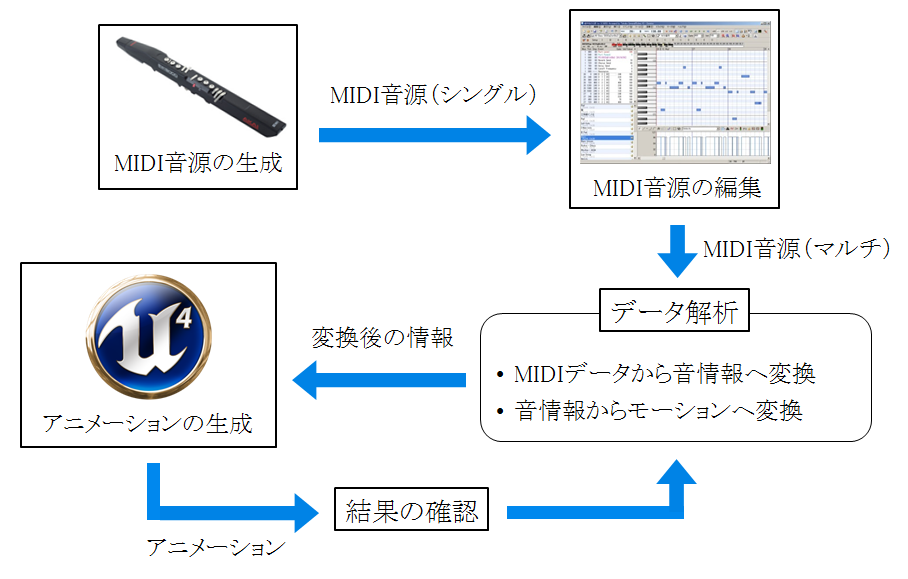
\includegraphics[width=14cm]{fig/chap3/flow.eps}
	\caption{音源から吹奏アニメーションを自動生成する流れ}
	\label{fig:flow}
\end{figure}
\\
\indent
実際のアニメーション制作フローに沿わせるため,音源の生成は電子楽器を用いて行う.
次に,生成した音源を解析し,譜面データへ変換する.
そして,アニメーション生成と同時に音源を流すことにより,音源に合わせてキャラクタが動くアニメーションを自動生成する.

\section{入力} \label{sec:input}
入力する音源は,MIDI音源とする.
ここで,MIDI音源は,MIDIという信号を用いて発音する音源のことである.
一般的に使用されるmp3やwaveなどの形式とは異なり,中身が譜面データとなっているため,音の解析が比較的容易である.
なお,MIDIの仕様は文献\cite{midi}に詳しく記載されている.\\
\indent
このMIDI音源を生成する方法は,\secref{sec:device}および\secref{sec:software}で説明する.

\section{出力} \label{sec:output}
出力は,管楽器を演奏するキャラクタのアニメーションである.
今回対象とする管楽器は,トランペット,トロンボーンである.
この2本の楽器は,吹奏楽ではとくに目立つ楽器であり,また3Dモデルが入手しやすかったために選んだ.

\section{デバイス} \label{sec:device}
MIDI音源を生成するために,電子楽器であるウインドシンセサイザ「EWI5000」(\figref{fig:ewi})を使用した.
このウインドシンセサイザは,さまざまな楽器の音を再現することが可能である.
\begin{figure}[h]
	\centering
	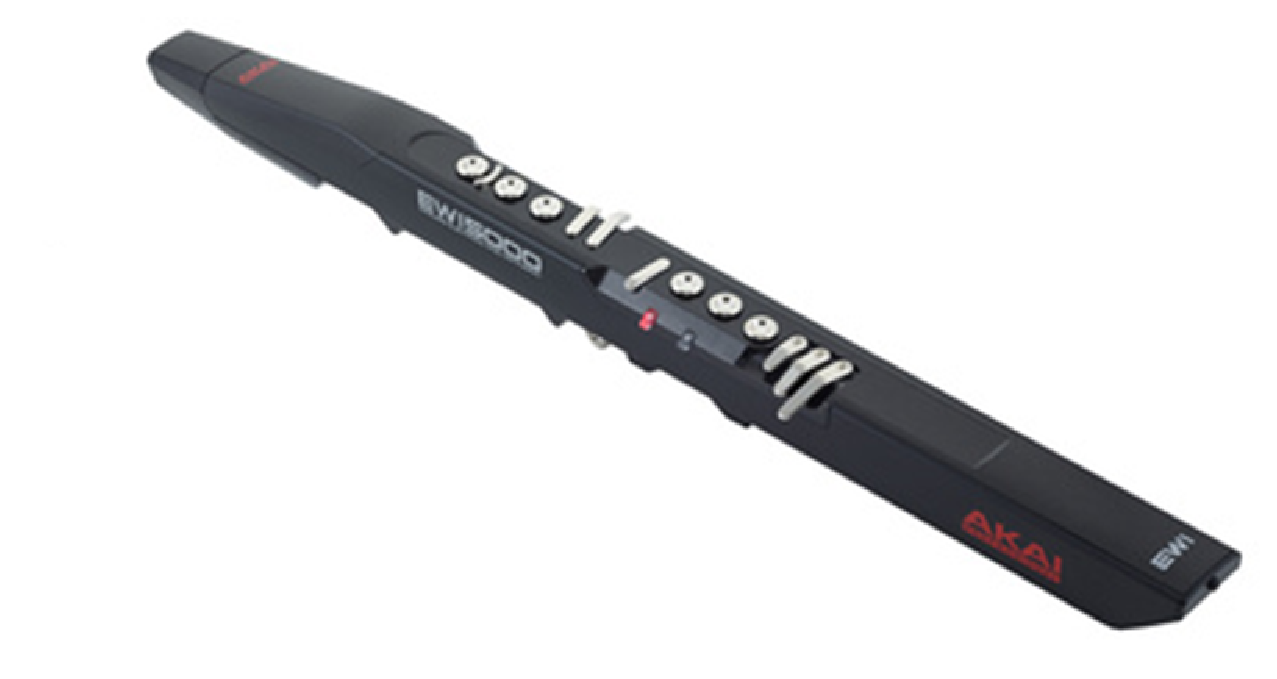
\includegraphics[width=10cm]{fig/chap3/ewi.eps}
	\caption{ウインドシンセサイザ「EWI5000」}
	\label{fig:ewi}
\end{figure}

\section{ソフトウェア} \label{sec:software}
\begin{figure}[h]
	\centering
	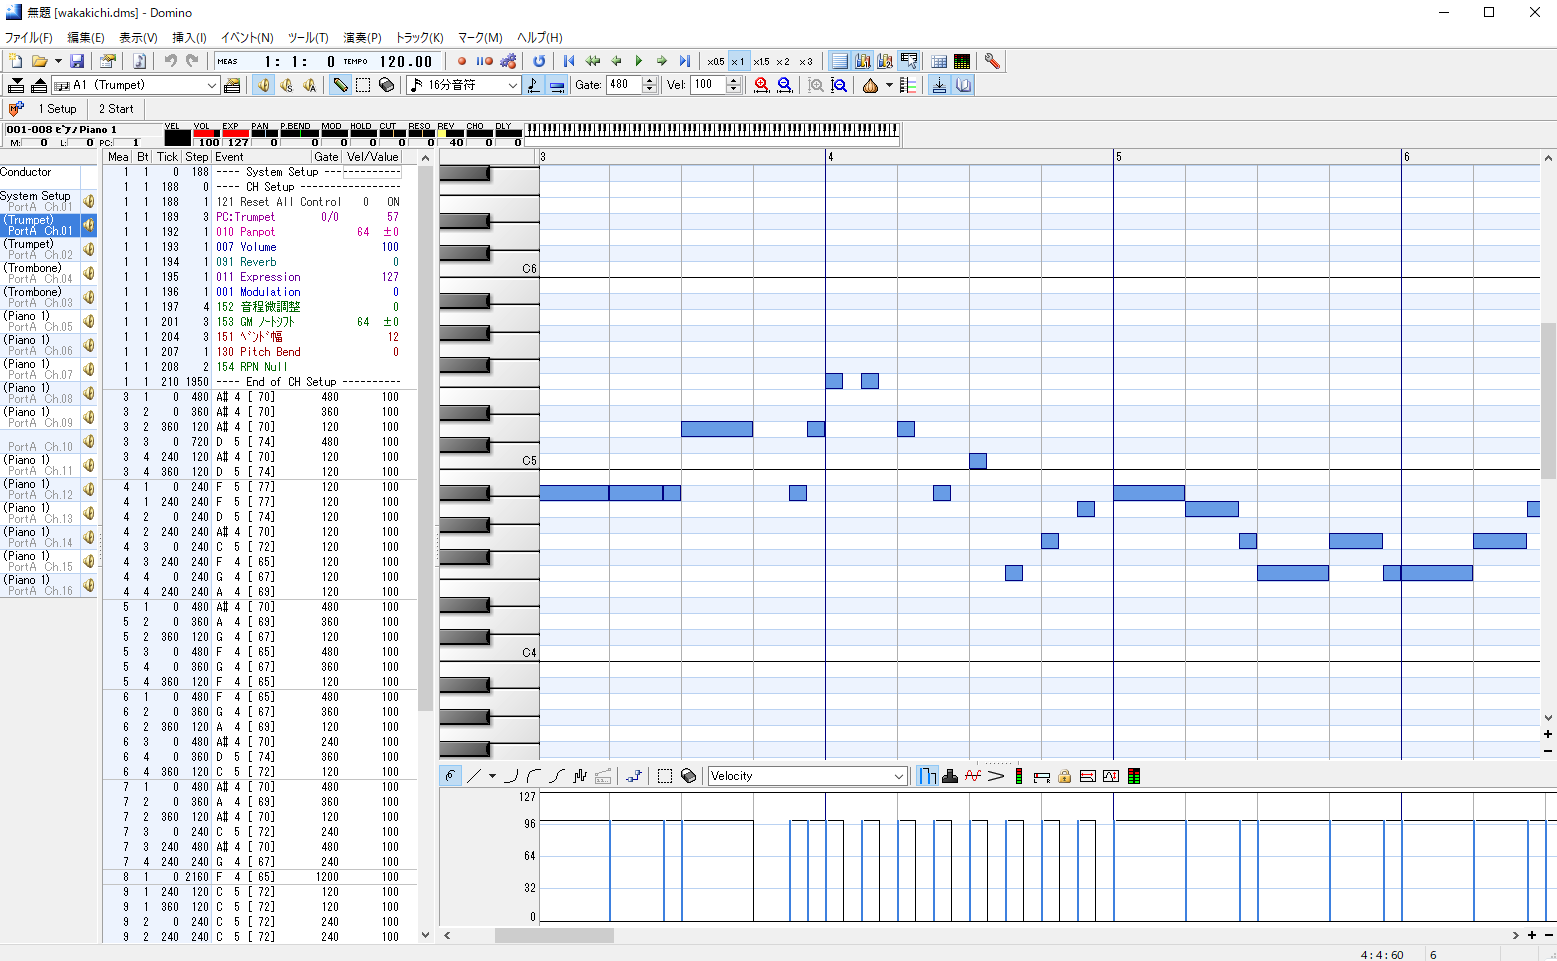
\includegraphics[width=10cm]{fig/chap3/domino.eps}
	\caption{MIDIシーケンスソフトウェア「domino」}
	\label{fig:domino}
\end{figure}
\secref{sec:device}で述べたウインドシンセサイザは,単音しか鳴らすことができないため,シングルチャンネルの音源しか生成することができない.
しかし,吹奏アニメーションを自動生成するためには,複数名で演奏しているマルチチャンネルの音源が必要となる.
そこで,ウインドシンセサイザで生成したMIDI音源を,フリーソフトウェアであるMIDIシーケンスソフトウェア「Domino」(\figref{fig:domino})\cite{domino}へ出力し,重ねて何度も録音することにより,マルチチャンネルの音源を生成した.\\
\indent
また,アニメーションの生成には,Epic Gamesより開発されたゲームエンジン,Unreal Engine\cite{ue4}を用いた.

\section{3Dモデル} \label{sec:3Dmodel}
使用する3Dモデルは,
ユニティちゃん(\subfigref{fig:model}{fig:unity}\cite{unity}),トランペット(\subfigref{fig:model}{fig:tp}\cite{tp}),トロンボーン(\subfigref{fig:model}{fig:tb}\cite{tb})である.
なお,ユニティちゃんのライセンス条約は,webサイト\cite{license}にて確認済みである.
\begin{figure}[h]
	\centering
	\subcaptionbox{\textgt{ユニティちゃん}
		\label{fig:unity}}[0.75\linewidth]{
		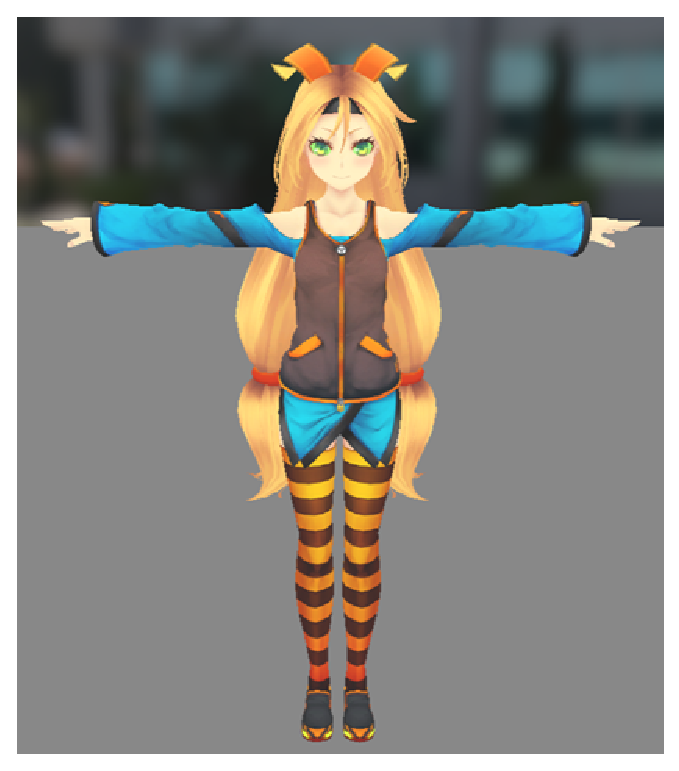
\includegraphics[height=7cm]{fig/chap3/unity.eps}}
	\subcaptionbox{\textgt{トランペット}
		\label{fig:tp}}{
		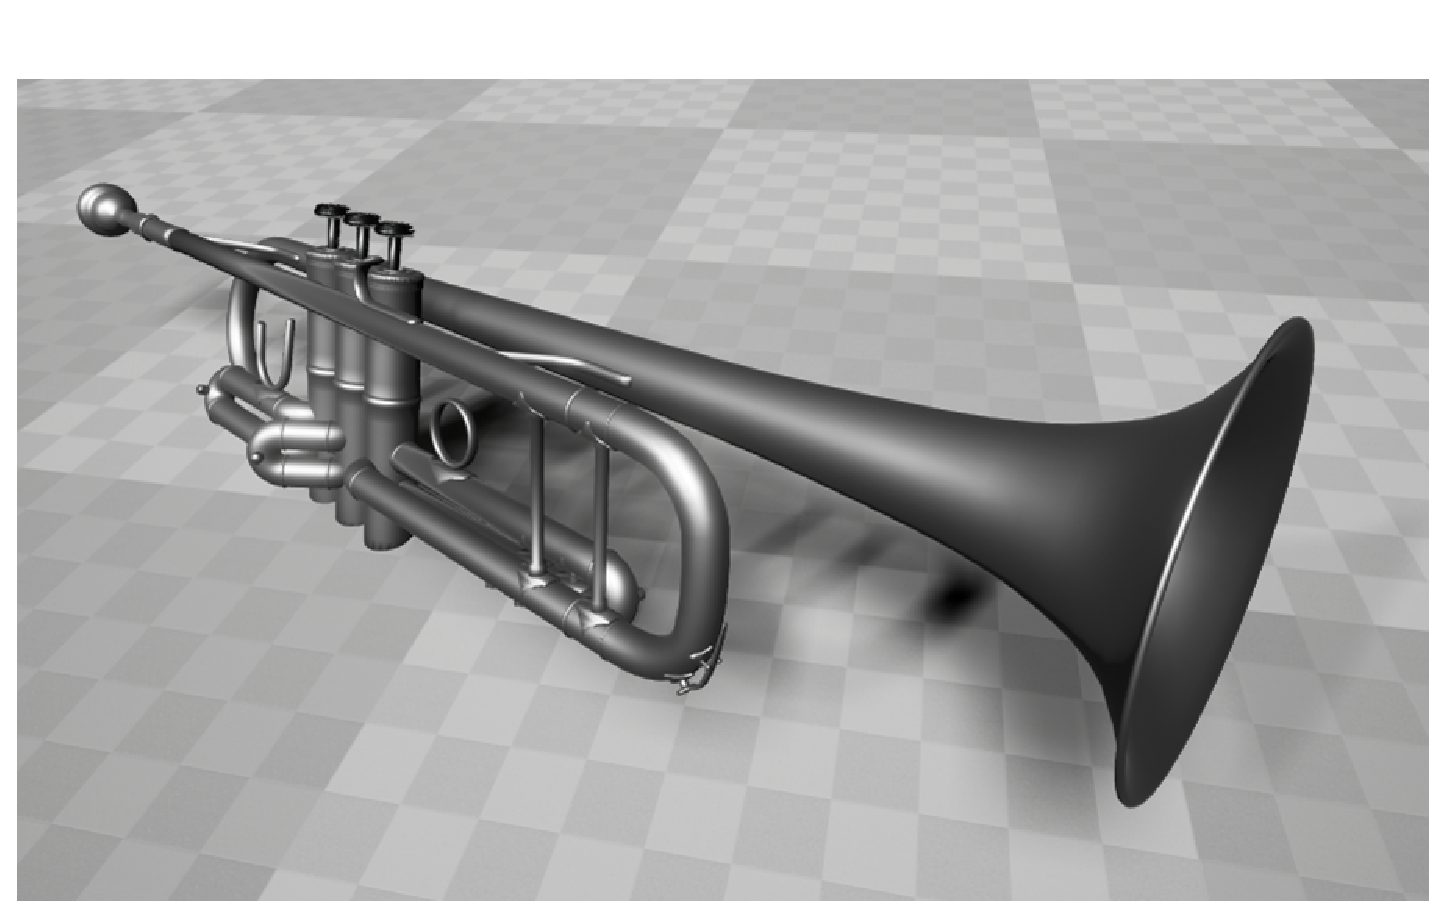
\includegraphics[width=6.5cm]{fig/chap3/tp.eps}}
	\subcaptionbox{\textgt{トロンボーン}
		\label{fig:tb}}{
		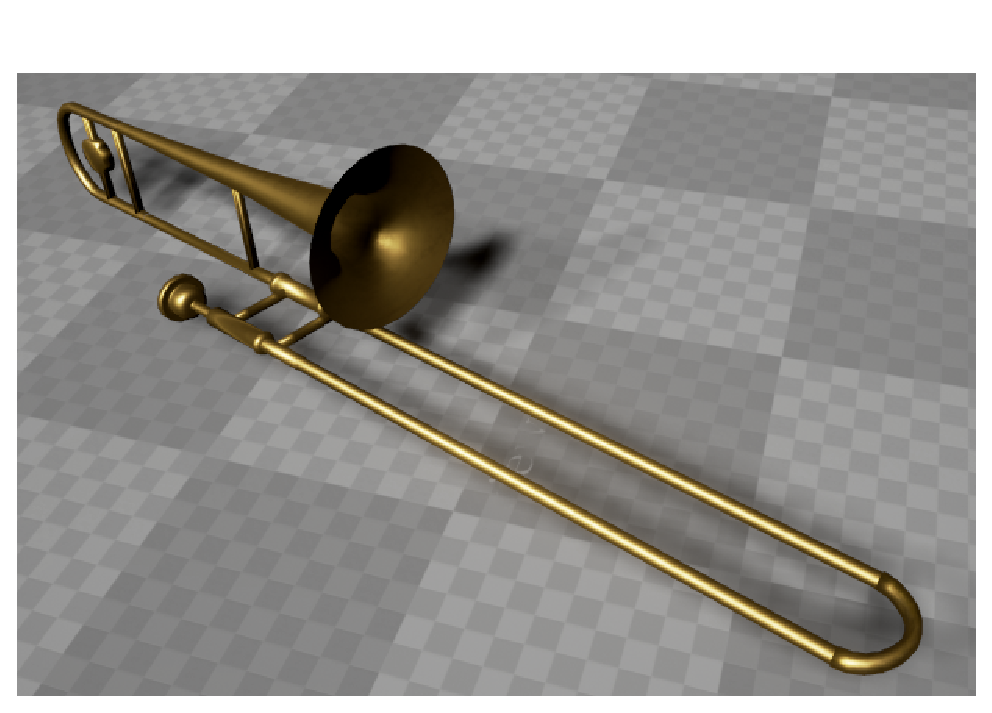
\includegraphics[width=7.5cm]{fig/chap3/tb.eps}}
	\caption{使用する3Dモデル}
	\label{fig:model}
\end{figure}
\newpage
\indent
ユニティちゃんは,主に以下の部位を制御する.
\begin{itemize}
	\item 右指(トランペット演奏時)
	\item 右腕(トロンボーン演奏時)
	\item 背
	\item 腰
	\item 両足
	\item 口元
\end{itemize}
\section{MIDIデータから音情報への変換} \label{sec:analysis}
MIDIは,チャンクとよばれるデータブロックから構成され,先頭にヘッダチャンク,その後にトラックチャンクが続く.
ヘッダチャンクには,チャンクタイプ,データ長さ,フォーマットタイプ,トラック数,タイムベース値という5つの値が格納されている.
ここで,タイムベース値とは,四分音符1つ分のクロック数を表す値であり,一般的には48から960までの自然数から,96の倍数が選ばれることが多い.
一方トラックチャンクには,チャンクタイプ,データ長,トラックイベントデータが格納されている.
提案手法では,トラック数,タイムベース値,トラックイベントデータを楽譜データに変換した後に,アニメーションに適用できる形へとさらに変更する.\\
\indent
まず,音に関する情報を楽譜データに変換する方法について説明する.
テンポ情報は,四分音符あたりの秒数($\mu$s)として格納されている.
音に関する情報は,トラックイベントデータとして,以下のように16進数で格納されている.\\

\hspace{10mm}9 0 4 8 6 4 8 1 7 0 8 0 4 8 0 0 8 3 6 0\\

この情報を2つずつペアにし,そこから音の種類と長さを取得する.
それぞれの数字から得られる情報は,以下の通りである.
\newpage
\begin{itemize}
	\item 90: ノートオン.このタイミングで音を鳴らすことを意味する.
	\item 48: 音の種類(48はドを意味する.対応表は次項に示す.)
	\item 64: 音の大きさ
	\item 81: 音を鳴らす長さ
	\item 70: 音を鳴らす長さ
	\item 90: ノートオフ.このタイミングで音を止めることを意味する.
	\item 48: 音の種類(48はドを意味する.)
	\item 00: 音の大きさ(音を止めているため,大きさはゼロとなる.)
	\item 83: 音を止める長さ
	\item 60: 音を止める長さ
\end{itemize}
\vspace{5mm}
音の長さは,以下のように取得する.ここでは,81 70を用いて説明する.
\begin{itemize}
	\item それぞれを2進数に変換する.\hspace{1mm}81: 1000 0001,70: 0111 0000
	\item それぞれの最上位ビットを取り除いて合成し,10進数に直す.\hspace{1mm}000 0001 111 0000 → 240
\end{itemize}
\vspace{5mm}
この例の場合,ドを240クロック分伸ばすことを意味する.以降,この値をデルタタイムとよぶ.
%デルタタイムを楽譜の情報に直すには,本節の冒頭で述べたタイムベース値を用いる.
最後に,このクロックを現実時間[s]に変換する.変換式は式\eqref{eq:eq1}で表される.\\
\begin{equation}
\label{eq:eq1}
時間[s] = 
\frac {デルタタイム[ticks] × 60[seconds/minute]}{タイムベース値[ticks/beat] * テンポ[beats/minute]}
\end{equation}
\\
タイムベース値,テンポをそれぞれ仮に480,120とすると,例で示した音情報は,譜面情報に直した結果『ドを0.25秒伸ばし,0.5秒休む』ことを意味すると分かる.
\newpage
\section{音情報のモーションへの適用} \label{sec:adapt}
\subsection{指や腕,楽器のパーツへの適用}
楽器を演奏する様子をアニメーションで再現するには,キャラクタの指や腕を介して楽器のモデルを制御する必要がある.
トランペットはピストンの操作,トロンボーンはスライドの操作により音を変えることができ,ピストンは3箇所,スライドは止める場所が大きく分けて7箇所ある.
トランペットのピストン番号を,吹き口に近い方から1-3(\subfigref{fig:numbering}{fig:piston}),トロンボーンのスライドの位置を,吹き口に近い方から1-7(\subfigref{fig:numbering}{fig:slide})と表すと,MIDIデータと音,運指の対応は\tabref{tab:map}となる.
\begin{figure}[h]
	\centering
	\subcaptionbox{\textgt{ピストン番号}
		\label{fig:piston}}{
		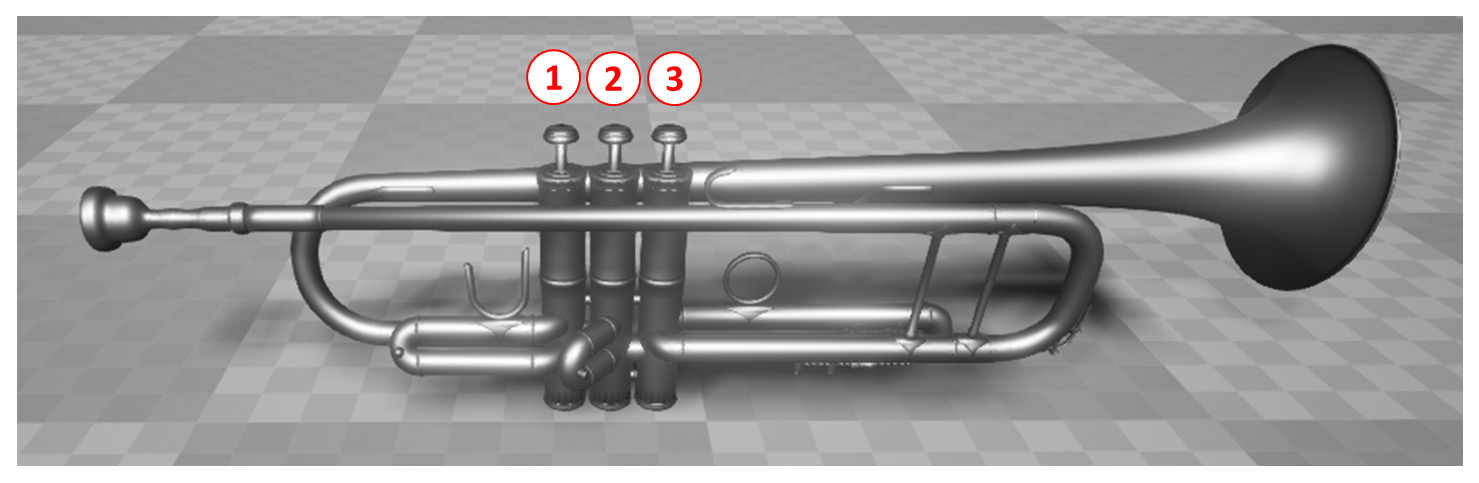
\includegraphics[width=10cm]{fig/chap3/tp_piston.eps}}
	\subcaptionbox{\textgt{スライドの位置番号}
		\label{fig:slide}}{
		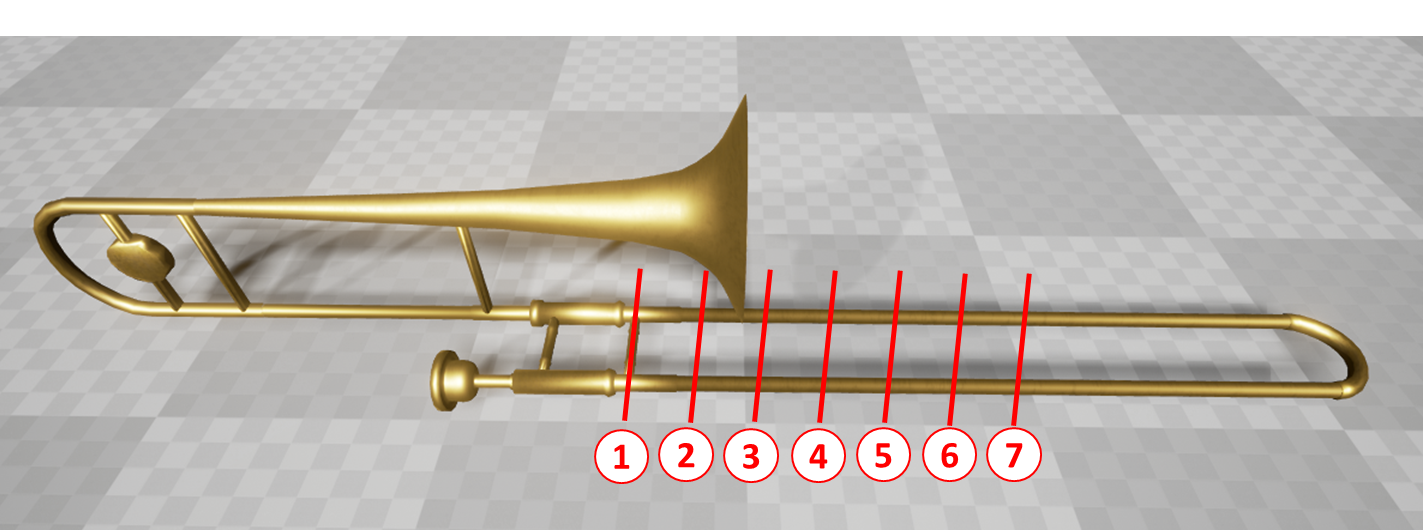
\includegraphics[width=13cm]{fig/chap3/tb_slide.eps}}
	\caption{トランペットのピストンおよびトロンボーンのスライドの番号付け}
	\label{fig:numbering}
\end{figure}

\begin{table}[h]
	\centering
	\caption{MIDIデータと音,運指の対応}
	\begin{tabular}{|c|c|c|c|} \hline
		MIDIデータ & 音名(実音) & トランペット & トロンボーン \\ \hline \hline
		\vdots & \vdots & \vdots & \vdots \\ \hline
		39 & A(ラ,442Hz) & 2 & 2 \\ \hline
		3b & B(シ) & 1・2・3 & 4 \\ \hline
		3c & C(ド) & 1・3 & 3 \\ \hline
		3e & D(レ) & 1・2 & 1 \\ \hline
		40 & E(ミ) & 2 & 2 \\ \hline
		41 & F(ファ) & 0 & 1 \\ \hline
		43 & G(ソ) & 1・2 & 2 \\ \hline
		45 & A(ラ) & 2 & 2 \\ \hline
		\vdots & \vdots & \vdots & \vdots \\ \hline
	\end{tabular}
	\label{tab:map}
\end{table}
\newpage
\secref{sec:analysis}で例として挙げた,『ドを0.25秒伸ばし,0.5秒休む』という譜形を演奏する場合,トランペットの場合は,1番と3番を0.25秒間押し続け,その後0.5秒間は休みのためそのまま,トロンボーンの場合は,スライドを3番まで移動させ,そのまま0.25秒間維持,その後0.5秒間は休みのためそのまま,という表現方法となる.\\

\newpage
\subsection{口元のメッシュへの適用}
\indent
金管楽器を演奏する際,高音域の演奏時は,低音域に比べて口元が緊張する.
緊張の程度には個人差があるが,本論文では,高音演奏時と低音演奏時の口元の違いを\figref{fig:mouth}のように,口の引き具合で表す.
\vspace{-2mm}
\begin{figure}[H]
	\centering
	\subcaptionbox{\textgt{低音域演奏時}
		\label{fig:low}}[0.45\linewidth]{
		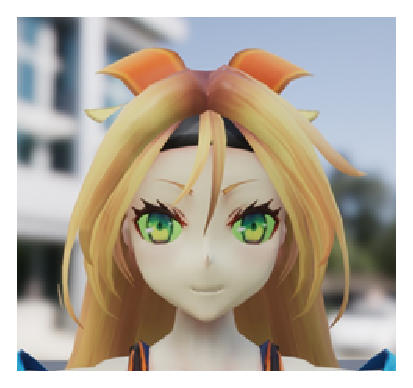
\includegraphics[width=6cm]{fig/chap3/low.eps}}
	\subcaptionbox{\textgt{高音域演奏時}
		\label{fig:high}}[0.45\linewidth]{
		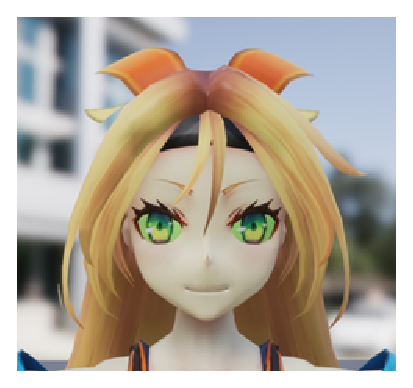
\includegraphics[width=6cm]{fig/chap3/high.eps}}
	\caption{音域による口元の変化}
	\label{fig:mouth}
\end{figure}
\indent
休みが一定の時間以上続く場合,演奏者は息継ぎを行う.息継ぎのタイミングには個人差があり,演奏しているフレーズによっても異なるが,提案手法では息継ぎのタイミングを以下の3パターンに分ける.
\begin{itemize}
	\item 休みが0.5拍以上~1拍未満: 休みの間,息継ぎのモーションを行う.
	\item 休みが1拍以上~2拍未満: 最後の1拍で息継ぎのモーションを行う.
	\item 休みが2拍以上: 最後の2拍間で,息継ぎの予備モーションおよび息継ぎのモーションを行う.
\end{itemize}

息継ぎのモーションを行うときに,口元を\figref{fig:breath_mouth}のように変形させる.
その他のモーションについては次項で述べる.\\
\vspace{-2mm}
\begin{figure}[!h]
	\centering
	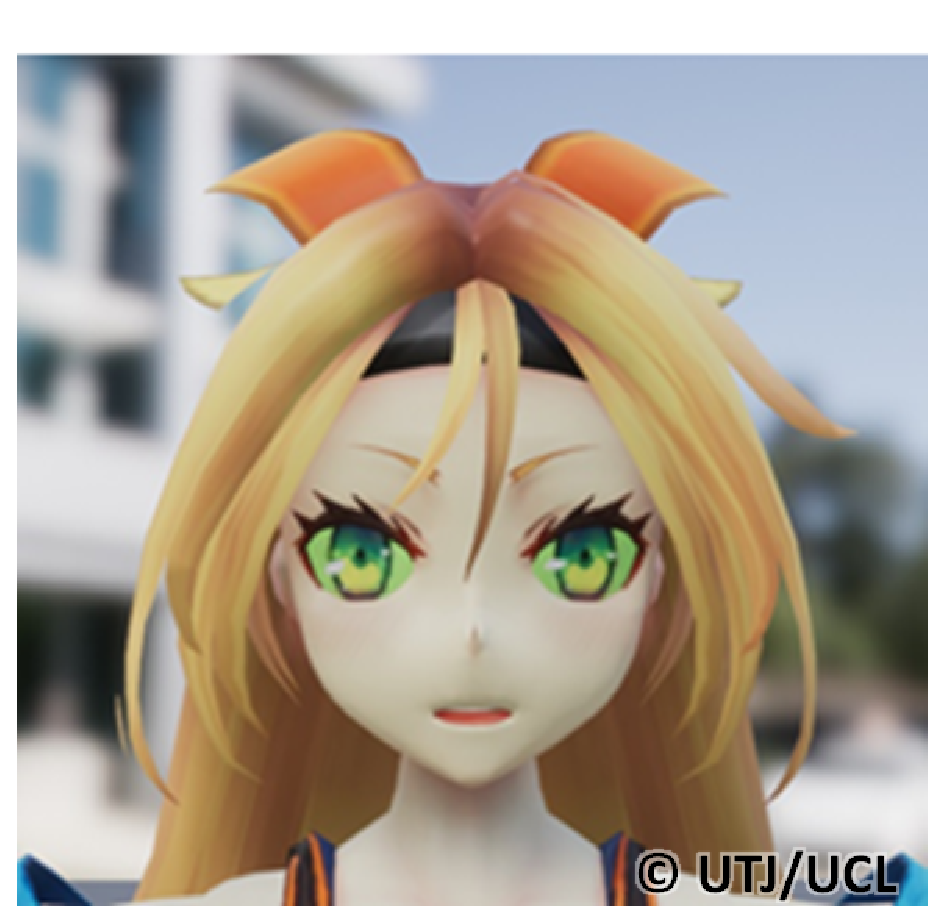
\includegraphics[width=6cm]{fig/chap3/breath.eps}
	\caption{息継ぎをするときの口元}
	\label{fig:breath_mouth}
\end{figure}
\newpage
\subsection{その他の部位への適用}
\indent
息継ぎをするときは口元だけでなく,上半身も動く.
そこで,前項で述べたタイミングで,
息継ぎのモーション(\subfigref{fig:breath_motion}{fig:breath_up}),
息継ぎの予備モーション(\subfigref{fig:breath_motion}{fig:breath_down})を行う.
なお,比較対象として通常の直立状態を\subfigref{fig:breath_motion}{fig:breath_default}に示す.差が分かりづらい場合は,楽器と床の端との位置関係を見てほしい.\\
\begin{figure}[!h]
	\centering
	\subcaptionbox{\textgt{息継ぎのモーションの最中}
		\label{fig:breath_up}}[0.45\linewidth]{
		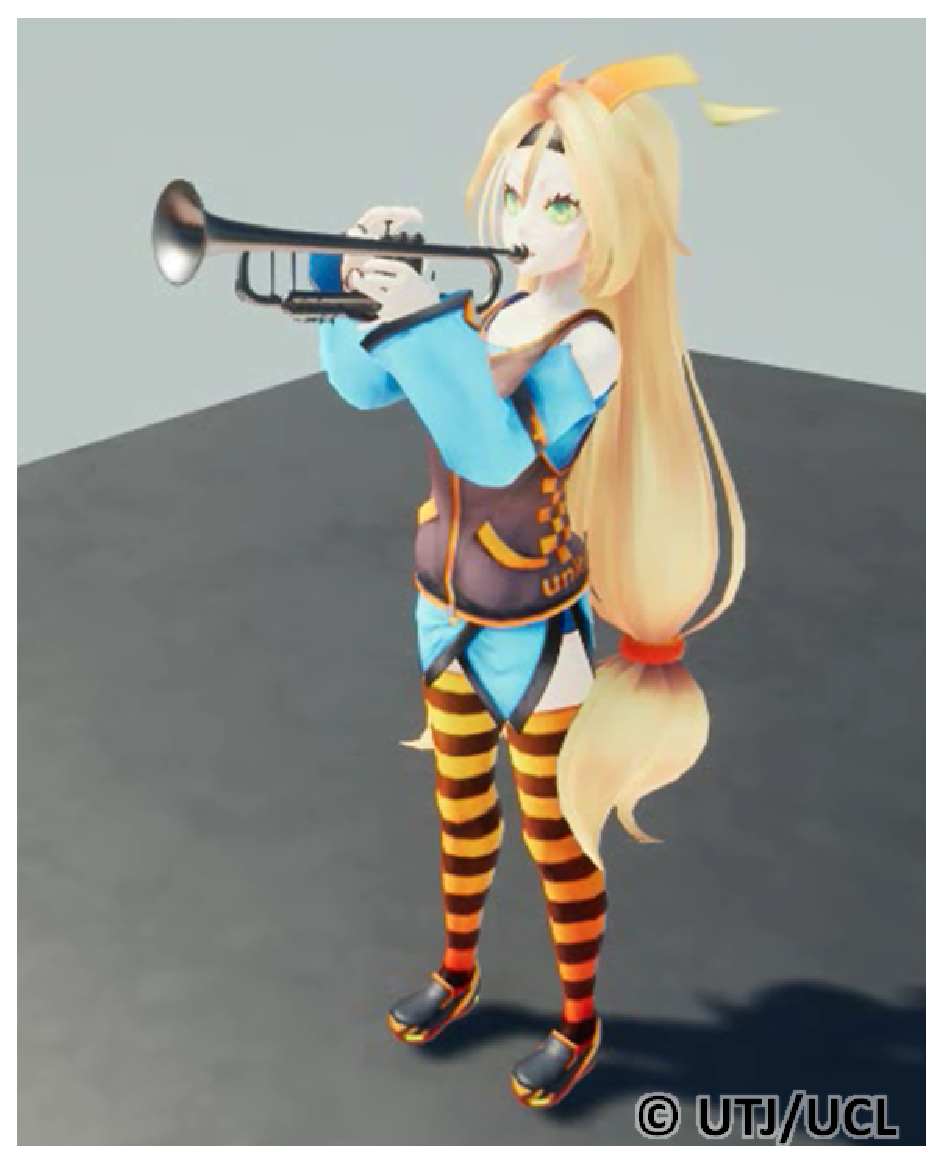
\includegraphics[width=6cm]{fig/chap3/up.eps}}
	\subcaptionbox{\textgt{息継ぎの予備モーションの最中}
		\label{fig:breath_down}}[0.45\linewidth]{
		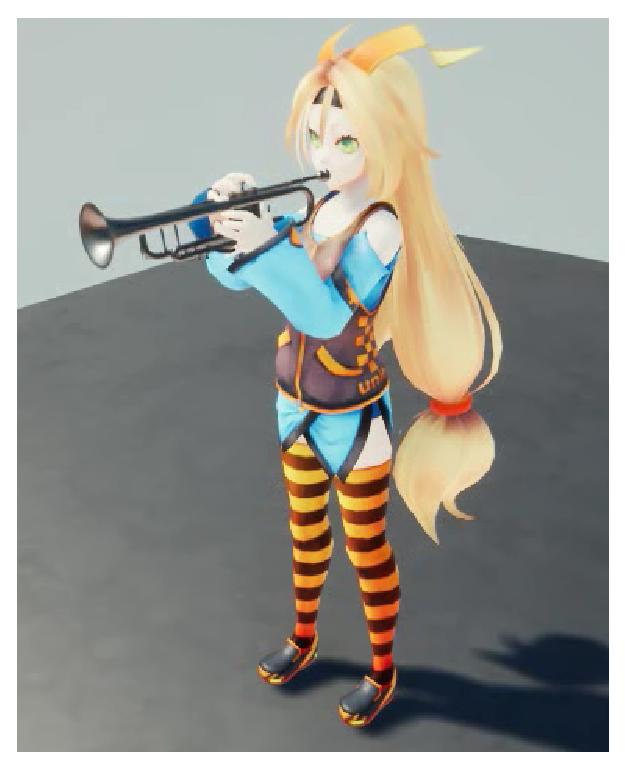
\includegraphics[width=6cm]{fig/chap3/down.eps}}
	\subcaptionbox{\textgt{通常の直立状態}
		\label{fig:breath_default}}[0.45\linewidth]{
		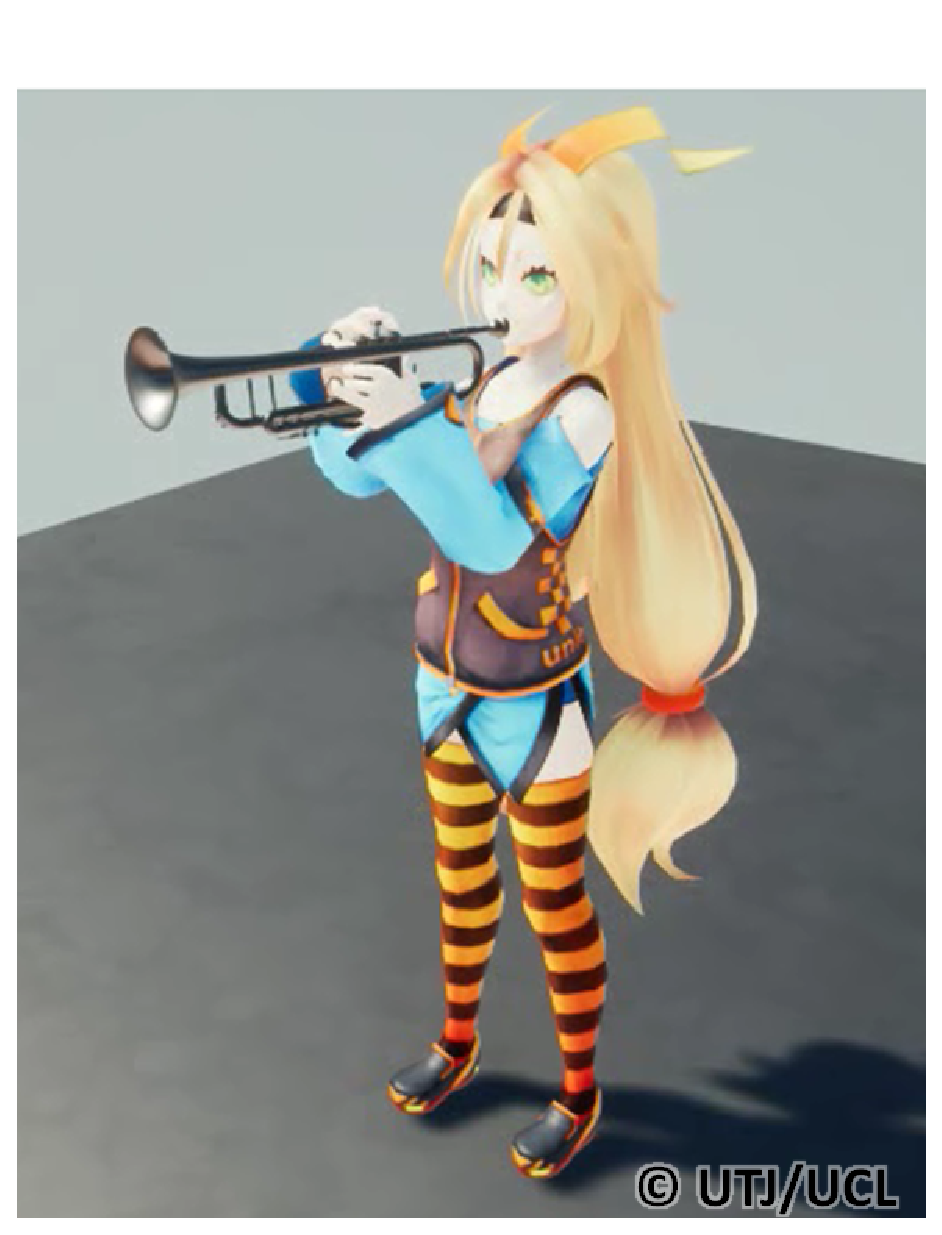
\includegraphics[width=6cm]{fig/chap3/default.eps}}
	\caption{息継ぎ時のモーション}
	\label{fig:breath_motion}
\vspace{10mm}
\end{figure}
\newpage
\indent
息継ぎ時以外にも演奏者は動く.
例えば,任意のタイミングで重心を移動させたり,テンポに合わせて身体や楽器を上下に揺らす.
しかし実際,演奏時の動きには個人差があるため,モーションの大きさを調節するためのパラメタを指定することによる個人差の表現が可能となっている.
%現在はランダムでパラメタが設定される仕様となっている.
アンサンブルアニメーションを自動生成する際は,全員に異なるパラメタをランダムで割り当てることにより,個人差を表現する.
ここで,アンサンブルとは複数名で演奏することを意味し,一般的には少人数で演奏することをさす.
アンサンブルには指揮者が存在しないため,曲の始まりは,リードを担当する演奏者が楽器や身体で合図をする.
なお,重心移動や合図のモーションは,武内が担当した.
%音情報から一意に定義可能なモーションは堀井.\\

\section{提案手法の使用方法} \label{sec:howto}
提案手法を用いてアニメーションを自動生成する際は,以下の順序が必要となる.
ここで,キャラクタや楽器のモデルは,あらかじめセッティングされているものとする.
\begin{enumerate}
	\item MIDI音源の作成
	\item 音源データの相対パスをソースコードに記載し,コンパイル
	\item Unreal Engineを起動
	\item 1.で生成した音源をBGMとして設定
	\item 再生
	\item 結果の確認および修正
\end{enumerate}\par
手順4.について,本来ならMIDI音源を解析すると同時に音を流すべきであるが,現在の実装ではそれが不可能となっているため,解析する音源とは別に,流す音源として新たに設定する必要がある.
また,このとき音のずれが生じる場合がある.その場合は,音源を流すタイミングの調節が必要となるが,一度調節をするだけでアニメーションと音は完全に同期する.